\renewcommand{\imagepath}{../20-fermiqp/img}

\chapter{FermiQP: a Fermion Quantum Processor}
In this chapter, the FermiQP quantum gas microscopy experiment is introduced. It is first presented as a platform for quantum simulations and quantum computing. Then the projected experimental setup is explained.

\section{A Versatile Microscope for Quantum Gases}
Within the last two decades, quantum gas microscopes have evolved into a well-proven and auspicious platform for exploring the nature of atoms in correlated systems and researching phenomena of quantum many-body and condensed matter physics. In these machines, atoms are laser-cooled to sub-\si[]{\micro\kelvin} temperatures and caught in regular patterns with the optical lattice technique. Single-site imaging techniques allow resolving individual atoms and detecting their respective states~\cite{bloch_many-body_2008,gross_quantum_2017, gross_quantum_2021}, granting access to the physics of their interactions. The underlying premise of this experimental approach is that for exploring the quantum realm, rather than simulating quantum phenomena on classical computers using established models of physics, which scale exponentially with the size of the described system, it is by far more advantageous to map these phenomena to controllable quantum systems and simulate them, as already suggested by Richard Feynman in 1982~\cite{feynman_simulating_1982}.

While the first quantum gas microscopes in the late 2000s were based on bosonic rubidium (e.g.~\cite{sherson_single-atom-resolved_2010}), for experiments using fermionic alkali atoms  first results were published in 2015, such as for potassium~\cite{cheuk_quantum-gas_2015} and lithium \cite{parsons_site-resolved_2015, omran_microscopic_2015}.

The FermiQP project, which started in 2021, is one of the newest fermion quantum gas microscopy experiments operated with lithium. It aims for surpassing existing fermionic lithium experiments with respect to their atom number, precision and atom lifetime in the microscope\todo{Really? Anything else}. It will combine two modes of operation: In the so-called \textit{analog mode}, FermiQP will use atoms in an optical lattice for investigating the nature of strongly interacting fermionic particles, which can be described by the Fermi-Hubbard model~\cite{hubbard_electron_1963, esslinger_fermi-hubbard_2010}. In the \textit{digital mode} on the other hand, FermiQP will act as a quantum computing platform exploiting the properties of its fermionic atoms and taking advantage of the long coherence time and the parallelizability of gate operations of atoms in optical lattices~\cite{zhang_functional_2022}. The key advantage over other platforms for quantum computing is the comparatively high scalability of quantum gases in optical lattices. The latter of both operation modes is what the experiment got its name from: a \text{Fermion Quantum Processor}.

FermiQP is a consortium of many contributing institutes and scientific groups in different areas of physics across Germany. The actual quantum gas microscope, the \textit{FermiQP demonstrator}, is being built at the Max Planck Institute of Quantum Optics in Garching, where this thesis was written.

The rest of this section introduces the techniques used in the FermiQP demonstrator and its projected features, followed by an overview of the planned experimental realization in the next section.

\subsection*{Laser Cooling}
Cooling and trapping of atoms with laser light is the necessary first step for a quantum gas microscope to run. With the idea dating back to the 1970s~\cite{hansch_cooling_1975}, it has paved the way for a whole realm of experiments exploring the world of atoms in ultracold regimes. After the 1997 nobel prize was awarded ``for development of methods to cool and trap atoms with laser light''\todo{citation}, they have become an established technique employed in a multitude of quantum gas experiments, which themselves have led to the 2001 nobel prize for achieving Bose-Einstein condensation\todo[]{citation}.

In the FermiQP demonstrator, different laser cooling techniques will be used: The atoms are first cooled and confined with a two- and a three-dimensional magneto-optical trap~\cite{foot_atomic_2005}, the latter of which is described in chapter~\ref{ch:mot}. Then gray molasses cooling~\cite{weidemuller_novel_1994} and evaporative cooling (see~\cite{foot_atomic_2005}, designed for FermiQP in~\cite{sun_construction_2022}), bring them into the (sub-) \si[]{\micro\kelvin} regime.

\subsection*{Optical Lattices}
Optical lattices are then used to confine cooled individual atoms into sites arranged in regular patterns. These patterns are created by standing waves of high-power laser beams creating repeated dipole potential wells at points with high intensity. The spacing of these wells is half the wave length of the lattice laser light. Using multiple lattice beams, arbitrary lattice geometries can be implemented by varying the angle of the beams to each other and their respective phase and power.Figures~\ref{fig:2d_lattice} and~\ref{fig:1d_lattice} illustrate how optical lattices confine atoms in regular patterns. In order not to drive transitions in the atom, the laser is very far red-detuned~\cite{bloch_many-body_2008, bloch_quantum_2012}.

In the FermiQP demonstrator, multiple lattices are going to be used. Most notably the science lattice at \SI[]{1064}{\nano\meter} laser wave length providing the two-dimensional regular pattern that the atoms are positioned in for the experiments, and the deeper pinning lattice with less distance between the lattice sites, ensuring that the atoms are well-confined when imaging light is shone in.

\begin{figure}
    \centering
    \begin{subfigure}[t]{0.3\textwidth}
        \centering
        \includegraphics[]{\imagepath/2d_lattice/2d_lattice.pdf}
        \caption{Visualization of a two-dimensional optical lattice with an atom in every site (image by Robin Groth)}
        \label{fig:2d_lattice}
    \end{subfigure}
    \hspace{0.03\textwidth}
    \begin{subfigure}[t]{0.3\textwidth}
        \centering
        \begin{tikzpicture}
            \begin{axis}[
                height=3.5cm,
                width=1.2\textwidth,
                xmin=-0.8, xmax=1.3,
                axis line style={draw=none},
                tick style={draw=none},
                xticklabels={,,}, yticklabels={,,}
            ]
                \addplot[thesisred, mark=none, line width=0.03cm, samples=500] {sin(2 * x*180)^2};
                \addplot[thesisgray, mark=*, only marks] coordinates {(-0.5, 0.2) (0.0, 0.2) (0.5, 0.2) (1.0, 0.2)};
            \end{axis}
        \end{tikzpicture}
        \caption{Optical lattice in one dimension}
        \label{fig:1d_lattice}
    \end{subfigure}
    \hspace{0.03\textwidth}
    \begin{subfigure}[t]{0.3\textwidth}
        \centering
        \begin{tikzpicture}
            \begin{axis}[
                height=3.5cm,
                width=1.2\textwidth,
                xmin=-0.8, xmax=1.3,
                axis line style={draw=none},
                tick style={draw=none},
                xticklabels={,,}, yticklabels={,,}
            ]
                \addplot[thesisred, mark=none, line width=0.03cm, samples=500] {0.5*sin(2 * x*180)^2 + 0.5*sin(x*180 + 45)^2};
                \addplot[thesisgray, mark=*, only marks] coordinates {(-0.45, 0.35) (-0.05, 0.35) (0.55, 0.35) (0.95, 0.35)};
            \end{axis}
        \end{tikzpicture}
        \caption{Example of an optical superlattice potential landscape in one dimension: Every other potential barrier is shallow, outlining a lattice of double-wells}
        \label{fig:1d_superlattice}
    \end{subfigure}
    \caption{Schematics of optical lattices}
    \label{fig:lattices}
\end{figure}

In FermiQP, the superlattice technique will be used: By overlapping the optical lattice with another lattice of double the lattice spacing, every other potential barrier between two sites can be lowered, creating a new lattice of double-wells. By varying the phase and amplitude of the lattice beams, different potential and barrier heights can be realized in the double-wells. This allows to control the tunneling rate between the sites of the double-well.

Raman sideband cooling will provide cooling for the atoms when they are confined in their lattice sites (see~\cite*{hilker_spin-resolved_2017}, designed for FermiQP in~\cite{krumm_notitle_2022}).

\subsection*{Imaging}
FermiQP will implement fluorescence imaging where light scattered by the atoms is used as an imaging signal and absorption imaging where the absorption of light reveals the position of individual atoms in the lattice. Two high-numerical aperture objectives will be used for collecting the imaging signal. In addition to observing positions, spin states of the atoms can be read out using spin-resolving detection techniques, e.g.~by spatially separating atoms of different spin state into the two double-well sites~\cite{boll_spin-_2016} or different layers across the lattice plane~\cite{koepsell_robust_2020} with magnetic fields like in a Stern-Gerlach experiment. An example of spin-resolved imaging is shown in figure~\ref{fig:absorption_image}.

\begin{figure}
    \centering
    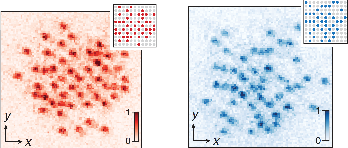
\includegraphics[]{\imagepath/imaging/imaging.pdf}
    \caption{Example of spin-resolving imaging (from~\cite{koepsell_robust_2020}): The two images show the position of spin-up and spin-down atoms in the lattice.}
    \label{fig:absorption_image}
\end{figure}

\subsection*{Quantum Simulations in the Analog Mode}
In the analog operation mode, the fermionc lithium atoms in the optical lattices are used for simulating phenomena of Fermi gases, such as the Mott insulator, superfluidity and  superconductivity, molecular phases of paired fermions, etc.~\cite{bloch_quantum_2012}. These phases emerge as different domains in the Fermi-Hubbard hamiltonian describing a system of fermions with spin state $\nu \in \{\Ket{\uparrow}, \Ket{\downarrow}\}$ in lattice sites $i$ and $j$~\cite{hubbard_electron_1963,esslinger_fermi-hubbard_2010}:
\begin{align}\label{eq:fermi_hubbard_hamiltonian}
    \hat H =
    \underbrace{-t \sum\limits_{\Braket{i,j}, \nu} \left(\hat a^\dagger_{i, \nu} \hat a_{j, \nu} + \text{h.c.}\right)}_\text{kinetic term/tunneling}
    + \underbrace{U \sum\limits_i \hat n_{i, \Ket{\uparrow}} \hat n_{i, \Ket{\downarrow}}}_\text{on-site interaction}
    + \underbrace{\sum\limits_{i, \nu} \epsilon_{i} \hat n_{i\, \nu}}_\text{offset}
\end{align}
with $\Braket{i,j}$ meaning that $i$ and $j$ are neighboring sites. The first term describes the rate of tunneling of a particle between two neighboring sites with the creation operator $\hat a^\dagger$ and the annihilation operator $\hat a$. The tunneling $t$ can be set in optical lattice experiments by lowering the potential barrier between sites, as hinted at above. The on-site interaction term describes the energy shift $U$ in sites where two atoms (in different spin states) are present, with $U > 0$ denoting repulsive and $U < 0$ denoting attractive interactions. The interaction between atoms on the same site is mediated by s-wave scattering. The mass of the particles and the free-space s-wave scattering length $a$ determine, along with other quantities, the interaction as $U \propto \frac{a}{m}$. The scattering length can be experimentally varied using Feshbach resonances as outlined in the next paragraph. Finally, $\epsilon_i$ is a site-dependent potential offset~\cite{esslinger_fermi-hubbard_2010}.

\begin{figure}
    \centering
    \begin{tikzpicture}
            \begin{axis}[
                height=5cm,
                width=0.8\textwidth,
                xmin=-0.8, xmax=1.35,
                axis line style={draw=none},
                tick style={draw=none},
                xticklabels={,,}, yticklabels={,,}
            ]
                \addplot[color=thesisred, mark=none, line width=0.06cm, samples=500] {sin(2 * x*180)^2};

                \addplot[color=thesisfuchsia, mark=*, mark size=0.14cm, only marks] coordinates {(-0.5, 0.2)};
                \addplot[color=thesisfuchsia, opacity=0.5, mark=*, mark size=0.14cm, only marks] coordinates {(0.0, 0.2)};

                \draw[yscale=1, ->] (axis cs:-0.5, 0.30) arc [radius=0.25, start angle=180, delta angle=90, end angle=0]; 
                \draw (axis cs: -0.25, 0.65) node {\small $t$};

                \addplot[color=thesisfuchsia, mark=*, mark size=0.14cm, only marks] coordinates {(1.0-0.05, 0.7)};
                \addplot[color=thesisblue, mark=*, mark size=0.14cm, only marks] coordinates {(1.0+0.05, 0.7)}; 
                \draw[<->] (1.25, 0.22) -- (1.25, 0.68) node[midway, right] {\small $U$};

                \draw[color=thesisgray, thin, dashed] (0.05, 0.2) --(1.25, 0.2);
                \draw[color=thesisgray, thin, dashed] (1.1, 0.7) --(1.25, 0.7);
            \end{axis}
    \end{tikzpicture}
    \caption{Tunneling and on-site interactions in the Fermi-Hubbard hamiltonian~\eqref{eq:fermi_hubbard_hamiltonian} in an optical lattice~\cite{esslinger_fermi-hubbard_2010}: The tunneling of a particle is determined by $t$, whereas the on-site interaction energy $U$ is the energy sites with two particles (of different spin state) are shifted by. Purple and blue colors indicate the spin state.}
    \label{fig:fermi_hubbard_schematic}
\end{figure}

\paragraph*{Feshbach Resonances} Feshbach resonances allow varying the scattering length $a$ of certain atoms by applying a constant magnetic field and so also the on-site interaction $U$ in the Fermi-Hubbard model. In the collision process of two atoms, this magnetic field sets the energy difference between two states of the atoms, a scattering state and a bound molecular state with different magnetic moments. At a certain magnetic field $B_0$, these energy levels coincide and the scattering length becomes infinite, which is a Feshbach resonance. For $B < B_0$, the scattering length is positive, $a > 0$, and $U$ is repulsive, whereas for $B > B_0$, one gets $a < 0$ and attractive $U$:
\begin{align}
    a = a_\text{background} \left(1 - \frac{\Delta}{B-B_0}\right)
\end{align}
with the width $\Delta$ of the Feshbach resonance and the background scattering length $a_\text{background}$ at the absence of a magnetic field. Fermionic lithium has a broad ($\Delta = \SI[]{300}{\gauss}$) resonance at $B_0 = \SI[]{834}{\gauss}$ allowing a large variation of the on-site interaction in the FermiQP demonstrator experiment~\cite{chin_feshbach_2010}.

\subsection*{Quantum Computing in the Digital Mode}
In the digital mode, FermiQP aims to serve as a platform for universal quantum computing. Quantum computers are supposed accelerate the execution of certain algorithms that scale exponentially with problem size on classical computer hardware in terms of their execution time, such are Shor's algorithm for factoring large numbers~\cite{shor_algorithms_1994}. Quantum computers make use of entanglement and superposition of states to achieve this speed-up. In quantum computers, the smallest unit of information is a so-called qubit, a two-level system of quantum states~\cite{mainzer_quantencomputer_2020}.\todo{more citations}

In the FermiQP demonstrator, qubits are encoded in the two energetically lowest hyperfine magnetic sublevels of the $2\text{s}^2\text{S}_{1/2}$ manifold, called $\Ket{1}$ and $\Ket{2}$. In the domain of high magnetic fields of \SIrange[]{500}{1000}{\gauss}, the magnetic sublevels of this manifold are separated by multiple \si[]{\giga\hertz}.\cite{gehm_properties_2003,wei_magnetic-field_2013}.

Universal quantum computers need to implement two kinds of gate operations: single-qubit gates for flipping indivudial qubits and two-qubit gates for entangling two qubits~\cite{mainzer_quantencomputer_2020}:\todo{more citations}

\paragraph*{Single-Qubit Gates}
Single-qubit gates in the FermiQP demonstrator are implemented with Raman transitions driven by an ultraviolet tweezer beam at \SI[]{323}{\nano\meter} allowing addressing single individual sites of the optical lattice. Due to its low mass, Raman transitions over the manifold between the two aforementioned qubit states are highly suppressed in  fermonic lithium~\cite{wei_magnetic-field_2013}. In the FermiQP demonstrator, transitions between the two qubit states are therefore implemented with a detour over the magnetic sublevel $\Ket{6}$ via global microwave and radio-frequency pulses, as explained in figure~\ref{fig:single_qubit_gates}.

\begin{figure}
    \centering
    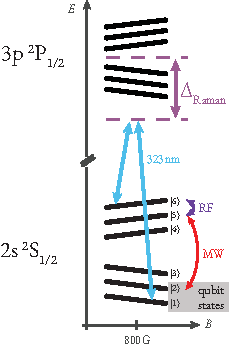
\includegraphics[]{\imagepath/single_qubit_gates/single_qubit_gates.pdf}
    \caption{Single qubit gate scheme in the FermiQP demonstrator (figure by Robin Groth): The states $\Ket{1}$ and $\Ket{2}$ in the the $2\text{s} ^2\text{S}_{1/2}$ manifold constitute a qubit.
    \SI[]{323}{\nano\meter} addressing beams couple $\Ket{1}$ with $\Ket{6}$ by a Raman transition via the $3\text{p} ^2\text{P}_{1/2}$ manifold. This Raman coupling can be driven selectively by focusing the \SI[]{323}{\nano\meter} beam onto individual sites of the optical lattice.
    A combination of a microwave (MW) and a radio-frequency (RF) pulse applied on all lattice sites couples $\Ket{2}$ and $\Ket{6}$ via $\Ket{5}$.\\
    A single qubit gate operation consists of an MW-RF pulse combination, then the Raman addressing, and another MW-RF pulse combination.
    In the addressed qubit, $\Ket{1}$ is coupled with $\Ket{6}$ via the Raman transition, which then is coupled to $\Ket{2}$ by the MW-RF pulses; $\Ket{2}$, on the other hand, is coupled by the MW-RF pulses to $\Ket{6}$, and then to $\Ket{1}$ via the Raman transition.
    All qubits that are not addressed by the Raman beam are preserved, as the two MW-RF pulse combinations bring the $\Ket{2}$ qubits back to their original state while the $\Ket{1}$ qubits are not stay unaffected.}
    \label{fig:single_qubit_gates}
\end{figure}

\paragraph*{Two-Qubit Gates}
Two-qubit operations in the FermiQP demonstrator will be implemented with collisional gates in double-wells of the superlattice. There two atoms are entangled by lowering the potential barrier and allowing interaction between them. The idea of two-qubit gates in optical lattices dates back more than two decades~\cite{jaksch_fast_2000, anderlini_controlled_2006,trotzky_time-resolved_2008,trotzky_controlling_2010}, collisional gates have recently gained even more interest with the maturing of quantum gas microscopy experiments~\cite{dai_generation_2016, yang_cooling_2020, zhang_functional_2022}.\todo{check and improve citations}

Arbitrary pairs of atoms can be entangled by moving them into neighboring lattice sites in the double-wells in the superlattice with optical tweezers, and then lowering the double-well barriers such that the atoms interact and entanglement is created, as depicted in figure~\ref{fig:two_qubit_gates}. These two-qubit gate operations can be achieved for multiple pairs of atoms in parallel by using multiple tweezers. Lowering the potential barrier is a global operation, hence all pairs of atoms in double-wells are entangled at the same time.

\begin{figure}
    \centering
    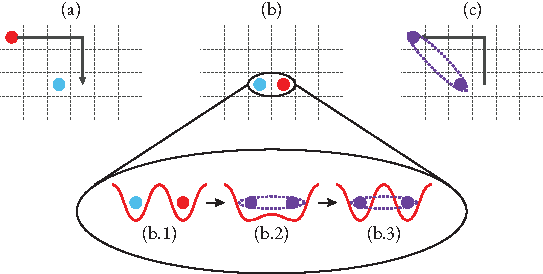
\includegraphics[]{\imagepath/two_qubit_gates/two_qubit_gates.pdf}
    \caption{Schematic of the two-qubit collisional gates in the FermiQP demonstrator: a: Two atoms that are supposed to be entangled are moved into neighboring sites using optical tweezers. b: The atoms are entangled by lowering the potential barrier in the double well (b.2) and letting the atoms interact. When the potential barrier is ramped up again, the entanglement (purple ellipse) is preserved. c: Then the atoms are moved to their original positions with the entanglement preserved.}
    \label{fig:two_qubit_gates}
\end{figure}



\section{Experimental Setup of the FermiQP Demonstrator}
\begin{figure}
    \centering
    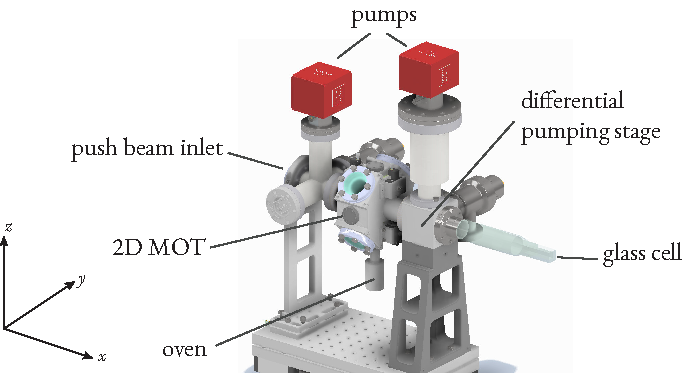
\includegraphics[]{\imagepath/chamber/chamber_side_0.pdf}
    \caption{Drawing of the planned design of the vacuum chamber: Atoms are evaporated from the over into the chamber of the two-dimensional magneto-optical trap (2D MOT) where the atoms are confined to a one-dimensional cloud. This cloud of atoms is then push along the $x$ axis through the differential pumping stage into the ultra-high vacuum region. There they reach the glass cell where they are captured by the three-dimensional magneto-optical trap. The axis set such that the atomic beam towards the glass cell runs along the $x$ axis, the $z$ axis points to the left as seen from the atomic beam, the $y$ axis points upwards.}
    \label{fig:chamber}
\end{figure}

\subsection*{Vacuum System}

\subsection*{Cooling Cycle}

\subsection*{Lithium-6}